\newcommand{\svcourse}{CST Part IA: Software Engineering and Security}
\newcommand{\svnumber}{1}
\newcommand{\svvenue}{Microsoft Teams}
\newcommand{\svdate}{2022-05-11}
\newcommand{\svtime}{15:00}
\newcommand{\svuploadkey}{CBd13xmL7PC1zqhNIoLdTiYUBnxZhzRAtJxv/ytRdM1r7qIfwMsxeVwM/pPcIo8l}

\newcommand{\svrname}{Dr Sam Ainsworth}
\newcommand{\jkfside}{oneside}
\newcommand{\jkfhanded}{yes}

\newcommand{\studentname}{Harry Langford}
\newcommand{\studentemail}{hjel2@cam.ac.uk}


\documentclass[10pt,\jkfside,a4paper]{article}

% DO NOT add \usepackage commands here.  Place any custom commands
% into your SV work files.  Anything in the template directory is
% likely to be overwritten!

\usepackage{fancyhdr}

\usepackage{lastpage}       % ``n of m'' page numbering
\usepackage{lscape}         % Makes landscape easier

\usepackage{verbatim}       % Verbatim blocks
\usepackage{listings}       % Source code listings
\usepackage{graphicx}
\usepackage{float}
\usepackage{epsfig}         % Embed encapsulated postscript
\usepackage{array}          % Array environment
\usepackage{qrcode}         % QR codes
\usepackage{enumitem}       % Required by Tom Johnson's exam question header

\usepackage{hhline}         % Horizontal lines in tables
\usepackage{siunitx}        % Correct spacing of units
\usepackage{amsmath}        % American Mathematical Society
\usepackage{amssymb}        % Maths symbols
\usepackage{amsthm}         % Theorems

\usepackage{ifthen}         % Conditional processing in tex

\usepackage[top=3cm,
            bottom=3cm,
            inner=2cm,
            outer=5cm]{geometry}

% PDF metadata + URL formatting
\usepackage[
            pdfauthor={\studentname},
            pdftitle={\svcourse, SV \svnumber},
            pdfsubject={},
            pdfkeywords={9d2547b00aba40b58fa0378774f72ee6},
            pdfproducer={},
            pdfcreator={},
            hidelinks]{hyperref}

\renewcommand{\headrulewidth}{0.4pt}
\renewcommand{\footrulewidth}{0.4pt}
\fancyheadoffset[LO,LE,RO,RE]{0pt}
\fancyfootoffset[LO,LE,RO,RE]{0pt}
\pagestyle{fancy}
\fancyhead{}
\fancyhead[LO,RE]{{\bfseries \studentname}\\\studentemail}
\fancyhead[RO,LE]{{\bfseries \svcourse, SV~\svnumber}\\\svdate\ \svtime, \svvenue}
\fancyfoot{}
\fancyfoot[LO,RE]{For: \svrname}
\fancyfoot[RO,LE]{\today\hspace{1cm}\thepage\ / \pageref{LastPage}}
\fancyfoot[C]{\qrcode[height=0.8cm]{\svuploadkey}}
\setlength{\headheight}{22.55pt}


\ifthenelse{\equal{\jkfside}{oneside}}{

 \ifthenelse{\equal{\jkfhanded}{left}}{
  % 1. Left-handed marker, one-sided printing or e-marking, use oneside and...
  \evensidemargin=\oddsidemargin
  \oddsidemargin=73pt
  \setlength{\marginparwidth}{111pt}
  \setlength{\marginparsep}{-\marginparsep}
  \addtolength{\marginparsep}{-\textwidth}
  \addtolength{\marginparsep}{-\marginparwidth}
 }{
  % 2. Right-handed marker, one-sided printing or e-marking, use oneside.
  \setlength{\marginparwidth}{111pt}
 }

}{
 % 3. Alternating margins, two-sided printing, use twoside.
}


\setlength{\parindent}{0em}
\addtolength{\parskip}{1ex}

% Exam question headings, labels and sensible layout (courtesy of Tom Johnson)
\setlist{parsep=\parskip, listparindent=\parindent}
\newcommand{\examhead}[3]{\section{#1 Paper #2 Question #3}}
\newenvironment{examquestion}[3]{
\examhead{#1}{#2}{#3}\setlist[enumerate, 1]{label=(\alph*)}\setlist[enumerate, 2]{label=(\roman*)}
\marginpar{\href{https://www.cl.cam.ac.uk/teaching/exams/pastpapers/y#1p#2q#3.pdf}{\qrcode{https://www.cl.cam.ac.uk/teaching/exams/pastpapers/y#1p#2q#3.pdf}}}
\marginpar{\footnotesize \href{https://www.cl.cam.ac.uk/teaching/exams/pastpapers/y#1p#2q#3.pdf}{https://www.cl.cam.ac.uk/\\teaching/exams/pastpapers/\\y#1p#2q#3.pdf}}
}{}


\usepackage{physics}
\usepackage{graphicx}
\usepackage{float}
\usepackage{wasysym}
\usepackage{amsfonts}

\begin{document}

\section{Example Sheet 1}

\begin{enumerate}

\item Given a dataset $\left(x_1,\ldots, x_n\right)$ we wish to fit a Poisson
distribution. This is a discrete random variable with a single parameter
$\lambda > 0$, called the rate, and

\[
\Pr\left( x ; \lambda \right) = \frac{\lambda^x e^{-\lambda}}{x!} \text{for}
 \ x \in\{0, 1, 2, \dots \}
\]

Show that the maximum likelihood estimator for $\lambda$ is $\hat{\lambda} =
n^{-1} \sum^{n}_{i=1} x_i$.

Since the throws are independent of each other, the probability of all of
them happening with a parameter $\lambda$ is given by:

\[
\begin{split}
\Pr(\left( x_1,\ldots, x_n \right) | \lambda) &= \prod^n_{i=1} \Pr(x_i |
\lambda) \\
&= \prod^n_{i=1} \frac{\lambda^{x_i}e^{-\lambda}}{x_i!} \\
&= \frac{\lambda^{\sum^{n}_{i=1} x_i}e^{-n\lambda}}{\prod^n_{i=1} x_i!} \\
\end{split}
\]

The maximum likelihood estimator $\hat{\lambda}$ for this can be found by
differentiating with respect to $\lambda$ and finding the maximum.

With $S = \sum^{n}_{i=1}x_i  $ and $P = \prod^n_{i=1} x_i! $

\[
\begin{split}
\dv{\Pr(\left( x_1,\ldots, x_n \right) | \lambda)}{\lambda}
&=
\frac{S \lambda^{S-1}e^{-n\lambda} - n\lambda^S e^{-n\lambda}}{P} \\
&=
\frac{(S - n\lambda)\lambda^{S-1}e^{-n\lambda}}{P} \\
\end{split}
\]

Setting this equal to 0 gives the equation:

\[
\begin{split}
0 &=
\frac{(S - n\lambda)\lambda^{S-1}e^{-n\lambda}}{P} \Longrightarrow \\
0 &= (S - n\lambda)\lambda^{S-1}e^{-n\lambda} \Longrightarrow \\
0 &= S - n\lambda \vee 0 = \lambda^{S-1}e^{-n\lambda} \Longrightarrow \\
\lambda &= \frac{S}{n} \vee \hat{\lambda} = 0 \\
\end{split}
\]

By definition of the Poisson distribution, $\lambda > 0$ hence
$\hat{\lambda} \neq 0$. We can therefore conclude that the maximum
likelihood estimator $\hat{\lambda} = \frac{S}{n} = \frac{\sum^n_{i=1}x_i}{n}$
as required.

\item Given a dataset $[3, 2, 8, 1, 5, 0, 8]$ we wish to fit a Poisson
distribution. Give code to achieve this fit, using \texttt{scipy.optimize.fmin}.

For this and all following code fragments I will assume the following imports:

\begin{lstlisting}[language=Python]

import numpy as np
import pandas as pd
import scipy.stats as stats
import scipy.optimize as opt
from sklearn.linear_model import LinearRegression

\end{lstlisting}

The following code finds the optimum value for the parameter. The value
found is $3.857153320312502$ and matches the value found using the
mathematical method.

\begin{lstlisting}[language=Python]

data = [3,2,8,1,5,0,8]

def logprob(x):
	return np.sum(stats.poisson.logpmf(data,x))

param = np.exp(opt.fmin(lambda x: -logprob(np.exp(x)),1))

\end{lstlisting}

\item The dataset in question 2 comes from counts of radioactive particle
emissions. The technician says that the counter's display is defective and
that any value larger than 20 just displays as 20. You therefore decide to
model the datapoints as a truncated Poisson distribution,

\[
\Pr(x; \lambda) =
\begin{cases}
\frac{\lambda^x e^{-\lambda}}{x!} & \text{if} \ x \in \{0, 1, \dots, 19\} \\
1 - \sum^{19}_{r=0}\frac{\lambda^r e^{-\lambda}}{r!} & \text{if} \ x = 20 \\
0 & \text{if} \ x > 20 \\
\end{cases}
\]

\begin{enumerate}

\item Your engineer friends thinks one should use unbiased estimators rather
than maximum likelihood estimators. Show that for the Poisson probability
model in question 1 the maximum likelihood estimator $\hat{\lambda} =
\frac{\sum^n_{i=1}x_i}{n}$ is unbiased.

Let $X$ be distributed with a Poisson distribution with parameter
$\frac{\sum^n_{i=1}}{n}$. $\mathbb{E}\left( X \right) = \frac{\sum^n_{i=1}}{n}$.
So the expectation of $n$ samples from this distribution is
$n\mathbb{E}\left( X \right) = n\frac{\sum^n_{i=1}}{n} = \sum^n_{i=1} x_i$.
This is the observed mean. Hence the maximum likelihood estimator
$\hat{\lambda}$ is also unbiased.

\item Explain why, for the dataset in question 2, $\hat{\lambda} =
\frac{\sum^n_{i=1}x_i}{n} $ is the maximum likelihood estimate for the
truncated Poisson model.

All the data in the dataset $[3, 2, 8, 1, 5, 0, 8]$ are strictly less than
20. For this domain, the truncated Poisson has the same probability density
function as the same probability density as the Poisson distribution.
Therefore the equation and derivation of the maximum likelihood estimator is
the same.

\item Show that $\hat{\lambda} = \frac{\sum^n_{i=1}}{n}$ is \textit{not} an
unbiased estimator in the truncated Poisson model.

Let $X$ be distributed according to the truncated Poisson distribution with
parameter $\frac{\sum^n_{i=1}x_i}{n}$

\[
\begin{split}
\mathbb{E}(X) &= \sum^{19}_{x=0} x\cdot\frac{\lambda^x e^{-x}}{x!} +
20\cdot\left( 1 - \sum^{19}_{x=0} \frac{\lambda^x e^{-x}}{x!} \right) \\
\frac{n\mathbb{E}(X)}{n} &< \sum^{\infty}_{x=0} x\cdot\frac{\lambda^x
e^{-\lambda}}{x!} \\
\mathbb{E}\left(\frac{\sum^n_{i=1}x_i}{n}\right) &< \lambda \\
\end{split}
\]

Therefore the expected value of of $\frac{\sum^n_{i=1}x_i}{n}$ for $x_i$
sampled from a truncated Poisson distribution is strictly less than the
parameter for the same truncated Poisson distribution. Therefore
$\frac{\sum^n_{i=1}x_i}{n}$ is not an unbiased estimator for the truncated
Poisson model.

\item Which do you think one should use, maximum likelihood estimators or
unbiased estimators. Why?

In the general case, I thin maximum likelihood estimators are best. They're
often easier to calculate numerically and usually give better results. Unbiased
estimators are not unique, many of them are very poor and have high bias.
Worse, in many discrete distributions, unbiased estimators don't exist.

\end{enumerate}

\item Given a dataset $(x_1, \dots, x_n)$, we wish to fit the Uniform$[0,
\theta]$ distribution, where $\theta$ is unknown. show that the maximum
likelihood estimator is $\hat{\theta} = \max_i x_i$.

The probability density function for parameter $X$ distributed with the
Uniform$[0, \theta]$ distribution (I will assume the distribution is discrete)
is given by:
\[
\Pr(X = x) =
\begin{cases}
\frac{1}{\theta + 1} & \text{if} \ x <= \theta \\
0 & \text{otherwise} \\
\end{cases}
\]

With $1_{\theta \geq x_i}$ as the indicator function for $\theta \geq x_i$;
the probability of observing the data $[3, 2, 8, 1, 5, 0, 8]$ is given by:
\[
\begin{split}
\Pr((x_1, \dots, x_n)) &= \prod^n_{i=1} \frac{1}{\theta} 1_{\theta \geq x_i} \\
&= \frac{1}{\theta^n} \prod^n_{i=1} 1_{\theta \geq x_i} \\
&= \frac{1}{\theta^n} 1_{\theta \geq \max_i x_i} \\
\end{split}
\]

Since the probability decreases as $\theta$ increases for all $\theta \geq
\max_i x_i$ and is 0 for $\theta < \max_i x_i$, we can see that the maximum
probability occurs at $\theta = \max_i x_i$.

\item Your company has two systems which it wishes to compare, $A$ and $B$.
It has asked you to compare the two, on the basis of performance
measurements $(x_1, \dots, x_m)$ from system $A$ and $(y_1, \dots, y_n)$
from system $B$. Any fool using Excel can just compare the averages,
$\bar{x} = \frac{\sum^m_{i=1}x_i}{m}$ and $\bar{y} =
\frac{\sum^n_{i=1}x_i}{n}$, but you are cleverer than that and will harness
the power of Machine Learning.

Suppose the $x_i$ are drawn from $X \sim \mathcal{N}(\mu, \sigma^2)$, and the
$y_i$ are drawn from $Y \sim \mathcal{N}(\mu + \delta, \sigma^2)$, and all
the samples are independent and $\mu$, $\delta$ and $\sigma$ are unknown.
Find maximum likelihood estimators for the three unknown parameters.

Using the probability density function for the Normal distribution, we can
write down the probability of observing the $x_i$ and $y_i$. We shall then
take the partial derivative by all variables at the same time and find the
value for which all the partial derivatives are 0 and verify this value is a
maxima. These will give us maximum likelihood estimators.

\[
\begin{split}
\Pr((x_1, \dots, x_m) \wedge (y_1, \dots, y_n)) &=
\prod^m_{i=1} \frac{1}{\sqrt{2\pi}\sigma}e^{-\frac{(x_i -\mu)^2}{2\sigma^2}}
\times \prod^n_{i=1} \frac{1}{\sqrt{2\pi}\sigma}e^{-\frac{(y_i -\mu -
\delta)^2}{2\sigma^2}} \\
&=
\frac{1}{\left(\sqrt{2\pi}\sigma\right)^{m + n}} e^{-\frac{\sum^m_{i=1}(x_i -
\mu)^2 + \sum^n_{i=1}(y_i - \mu - \delta)^2}{2\sigma^2}} \\
\end{split}
\]

\[
\begin{split}
\pdv{\Pr}{\mu} &= \frac{\left(\sum^m_{i=1}(x_i - \mu) + \sum^n_{i=1}(y_i -
\mu - \delta)\right)}{\sigma^2}\frac{1}{\left(\sqrt{2\pi}\sigma\right)
^{m + n}} e^{-\frac{\sum^m_{i=1}(x_i -\mu)^2 + \sum^n_{i=1}(y_i - \mu - \delta)
^2}{2\sigma^2}} \\
&= \frac{\sum^{m}_{i=1} x_i + \sum^{n}_{i=1} y_i - (m + n)\mu - n\delta}
{\sigma^2}\frac{1}{\left(\sqrt{2\pi}\sigma\right)^{m + n}}
e^{-\frac{\sum^m_{i=1}(x_i -\mu)^2 + \sum^n_{i=1}(y_i - \mu - \delta)
^2}{2\sigma^2}} \\
0 &= \sum^{m}_{i=1} x_i + \sum^{n}_{i=1} y_i - (m + n)\mu - n\delta \\
\end{split}
\]

\[
\begin{split}
\pdv{\Pr}{\delta} &= \frac{\sum^n_{i=1}\left(y_i - \mu - \delta \right)
}{\sigma^2}\frac{1}{\left(\sqrt{2\pi}\sigma\right)^{m + n}} e^{-\frac{
\sum^m_{i=1}(x_i - \mu)^2 + \sum^n_{i=1}(y_i - \mu - \delta)^2}{2\sigma^2}} \\
&= \frac{\sum^n_{i=1} y_i - n\delta - n\mu}{\sigma^2}
 \frac{1}{\left (\sqrt{2\pi}\sigma\right)^{m + n}} e^{-\frac{\sum^m_{i=1}(x_i -
\mu)^2 + \sum^n_{i=1}(y_i - \mu - \delta)^2}{2\sigma^2}} \\
0 &= \sum^n_{i=1} y_i - n\delta - n\mu\\
\end{split}
\]

\[
\begin{split}
\pdv{\Pr}{\sigma} &= \left( \frac{\sum^m_{i=1}(x_i - \mu)^2 + \sum^n_{i=1}
(y_i - \mu - \delta)^2}{\sigma^3} - \frac{m + n}{\sigma} \right)
\frac{1}{\left (\sqrt{2\pi}\sigma\right)^{m + n}} e^{-\frac{\sum^m_{i=1}(x_i -
\mu)^2 + \sum^n_{i=1}(y_i - \mu - \delta)^2}{2\sigma^2}} \\
0 &= \sum^m_{i=1}(x_i - \mu)^2 + \sum^n_{i=1} (y_i - \mu - \delta)^2 - (m +
n)\sigma^2
\end{split}
\]

We can subtract the second expression from the first to get:
\[
\begin{split}
0 - 0 &= \sum^{m}_{i=1} x_i + \sum^{n}_{i=1} y_i - m\mu - n\mu - n\delta
+ n\delta + n\mu - \sum^{n}_{i=1} y_i \\
0 &= \sum^{m}_{i=1} x_i - m\mu\\
\hat{\mu} &= \frac{\sum^m_{i=1} x_i}{m} \\
\end{split}
\]

We can then substitute this result into the second expression to get:
\[
\begin{split}
0 &= \sum^n_{i=1} y_i - n\delta - n\mu\\
0 &= \sum^n_{i=1} y_i - n\delta - \frac{n\sum^m_{i=1} x_i}{m}\\
n\delta &= \sum^n_{i=1} y_i - \frac{n\sum^m_{i=1} x_i}{m} \\
\hat{\delta} &= \frac{\sum^n_{i=1} y_i}{n} - \frac{\sum^m_{i=1} x_i}{m} \\
\end{split}
\]

Substituting these values into the expression for $\sigma$ gives:

\[
\begin{split}
0 &= \sum^m_{i=1}(x_i - \mu)^2 + \sum^n_{i=1} (y_i - \mu - \delta)^2 - (m +
n)\sigma^2 \\
(m + n)\sigma^2 &= \sum^m_{i=1}\left( x_i - \frac{\sum^m_{i=1}x_i}{m}
\right)^2 + \sum^n_{i=1}\left( y_i - \frac{\sum^n_{i=1}y_i}{n} \right)^2 \\
\hat{\sigma}^2 &= \frac{\sum^m_{i=1}\left( x_i - \frac{\sum^m_{i=1}x_i}{m}
\right)^2 + \sum^n_{i=1}\left( y_i - \frac{\sum^n_{i=1}y_i}{n} \right)^2}{m
+ n} \\
\end{split}
\]

\item Let $x_i$ be the population of city $i \in \{1, \dots, n\}$, and let
$y_i$ be the number of crimes reported. Consider the model $Y_i \sim
\text{Poisson}(\lambda x_i)$, where $\lambda > 0$ is an unknown parameter.
Find the maximum likelihood estimator $\hat{\lambda}$.

Assuming that the number of crimes in each city are unrelated, under the
proposed model the probability of observing the number of crimes we have is
given by:

\[
\begin{split}
\Pr((y_1, \dots, y_n) | \lambda) &=
\prod^n_{i=1} \frac{\left( \lambda x_i \right)^{y_i} e^{-\lambda x_i}}{y_i
!} \\
&= \lambda^{\sum^n_{i=1}y_i}e^{-\lambda\sum^n_{i=1}x_i} \prod^n_{i=1}
\frac{x_i^{y_i}}{y_i!} \\
\end{split}
\]

We can differentiate this with respect to $\lambda$ and solve for 0
derivative to find the maximum likelihood estimator $\hat{\lambda}$.

\[
\begin{split}
\pdv{\Pr}{\lambda} &=
\left(\lambda^{\left( \sum^n_{i=1}y_i \right) - 1}\sum^n_{i=1}y_i -
\lambda^{\left( \sum^n_{i=1}y_i \right)}\sum^n_{i=1} x_i\right)e^{-\lambda
\sum^n_{i=1}x_i } \prod^n_{i=1}\frac{x_i^{y_i}}{y_i!} \\
&= \left( \sum^n_{i=1}y_i - \lambda\sum^n_{i=1} x_i\right) \lambda^{\left(
\sum^n_{i=1}y_i \right)- 1}e^{-\lambda\sum^n_{i=1}x_i }
\prod^n_{i=1}\frac{x_i^{y_i}}{y_i!} \\
0 &= \sum^n_{i=1}y_i - \hat{\lambda}\sum^n_{i=1} x_i \\
\hat{\lambda} &= \frac{\sum^n_{i=1}y_i}{\sum^n_{i=1} x_i} \\
\end{split}
\]

\item We wish to fit a piecewise linear line to a dataset, as shown below.
The inflection point is given, and we wish to estimate the slopes and
intercepts. Explain how to achieve this using a linear modelling approach.

The equation of a line which passes through a point $(x', y')$ can be given by:
$y = m(x - x') + y'$. We must fit two of those. This can be done with an
indicator variable, two gradients and a one-hot encoding. Note that we have
no intercepts since we know a point the line passes through.

\[
y \approx m_1 (x - x') 1_{x \leq x'} + m_2 (x - x') 1_{x > x'} + y'
\]

\begin{lstlisting}[language=Python]

"""
xp, yp is the inflection point
x, y are the x and y coordinates of the data
"""

features = ((x - xp) * [x <= xp, x > xp]).transpose()

model = LinearRegression(fit_intercept=False).fit(features, y - yp)

\end{lstlisting}

\item For the climate data from section 2.2.5 of the lecture notes, we
proposed the model

\[
\text{temp} \approx \alpha + \beta_1\sin(2\pi t) + \beta_2\cos(2\pi t) +
\gamma t
\]

in which the $+\gamma t$ term asserts that temperatures are increasing at a
constant rate. We might suspect though that temperatures are increasing
non-linearly. To test this, we can create a non-numerical feature out of t by

\begin{center}
\texttt{u = ``decade\_'' + str(math.floor(t/10)) + ``0s''}
\end{center}

and fit the model

\[
\text{temp} \approx \alpha + \beta_1\sin(2\pi t) + \beta_2\cos(2\pi t) +
\gamma_u
\]

Write this as a linear model, and give code to fit it.

The linear is:

\[
\text{temp} \approx \beta_1\sin(2\pi t) + \beta_2\cos(2\pi t) +
\gamma_{1950s}1_{1950s} + \dots + \gamma_{2020s}1_{2020s} + \mathcal{N}(0, \sigma)
\]

Where $\gamma_{XYZ0s}$ is the average temperature in decade $XYZ$, and
$1_{XYZ0s}$ is the indicator variable as to whether this temperature is in
the decade $XYZ$.

% verified that this fits well

\begin{lstlisting}[language=Python]

url = "https://.../climate.csv"
climate = pd.read_csv(url)
df = climate.loc[climate.station == "Cambridge"]
t = df.yyyy + (df.mm - 1) / 12
temp = (df.tmin + df.tmax) / 2
features = np.empty((10, t.size))
features[0] = np.sin(2 * np.pi * t)
features[1] = np.cos(2 * np.pi * t)
features[2:] = [t // 10 == i for i in range(195, 203)]

features = features.transpose()

LinearRegression(fit_intercept=False).fit(features, temp)

\end{lstlisting}

\item I have two feature vectors

\begin{align*}
\text{gender} = [f, f, f, f, m, m, m] & \text{eth} = [a, a, b, w, a, b, b]
\end{align*}

and I one-hot encode them as

\begin{align*}
g_1 &= [1, 1, 1, 1, 0, 0, 0] & & & e_1 &= [1, 1, 0, 0, 1, 0, 0] \\
g_2 &= [0, 0, 0, 0, 1, 1, 1] & & & e_2 &= [0, 0, 1, 0, 0, 1, 1] \\
	&						 & & & e_3 &= [0, 0, 0, 1, 0, 0, 0] \\
\end{align*}

Are these five vectors $\{g_1, g_2, e_1, e_2, e_3\}$ linearly independent?
If not, find a linearly independent set of vectors that spans the same
feature space.

The vectors $\{g_1, g_2, e_1, e_2, e_3\}$ are not linearly independent. The
following dependencies exist:

\[
\begin{split}
g_2 &= \mathbf{1} - g_2 \\
e_3 &= \mathbf{1} - e_1 - e_2 \\
\end{split}
\]

We can remove these dependencies by considering only the set of
$\{g_1, g_2, e_1, e_2, e_3\}$.

So the vectors we use are:

\begin{align*}
g_1 &= [1, 1, 1, 1, 0, 0, 0] & & & e_1 &= [1, 1, 0, 0, 1, 0, 0] \\
	&						 & & & e_2 &= [0, 0, 1, 0, 0, 1, 1] \\
\end{align*}

\item For the police stop-and-search dataset in section 2.6, we wish to
investigate intersectionality in police bias. We propose the linear model

\[
1[\text{outcome}=\text{``find''}] \approx \alpha_{\text{gender}} +
\beta_{\text{eth}}
\]

Write this as a linear model using one-hot coding. Are the parameters
identifiable? If not, rewrite the model so they are and interpret the
parameters of your model.

\[
1[\text{outcome}=\text{``find''}] \approx \alpha_1 g_1 + \beta_1 e_1 +
\beta_2 e_2 + \gamma
\]

The features are identifiable. $\gamma$ is the rate for a white male.
$\alpha_1$ is the difference between the male gender and the female gender,
$\beta_1$ is the difference between white ethnicity and asian ethnicity and
$\beta_2$ is the difference between white ethnicity and black ethnicity.

\end{enumerate}

\section{Supplementary Questions}

\begin{enumerate}[label=\arabic*]

\setcounter{enumi}{10}

\item Fit the model

\[
\text{Petal.length} \approx \alpha - \beta(\text{Sepal.length})^{\gamma},
\gamma > 0
\]

by minimizing the mean square error.

\begin{lstlisting}[language=Python]

url = "https://.../iris.csv"
iris = pd.read_csv(url)

def pred(x):
	return x[0] - x[1] * np.power(iris['Sepal.Length'], np.exp(x[2]))

def mean_squared_error(x):
	return np.sum(np.power(iris['Petal.Length'] - pred(x), 2))

opt.fmin(mean_squared_error, [-1.385e5, -1.385e5, -9.5])

\end{lstlisting}

\begin{figure}[H]
\centering
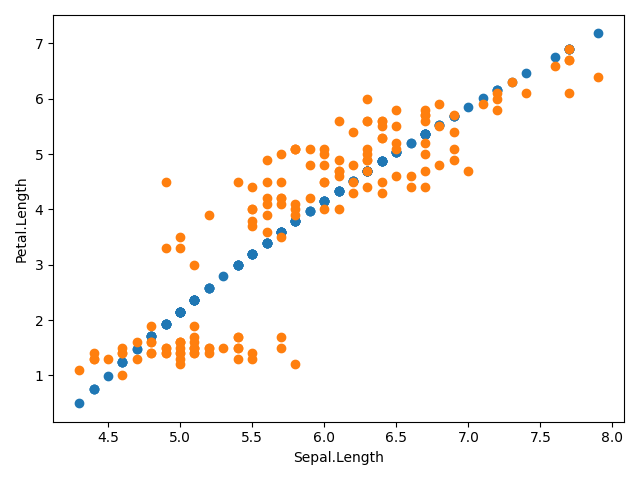
\includegraphics[width=0.5\textwidth]{./q7_sepaltopetal}
\end{figure}

\item As an alternative to the model from question 8, we might suspect that
temperatures are increasing linearly up to 1980, and that they are
increasing linearly at a different rate from 1980 onwards. Devise a linear
model to express this, using your answer to question 7, and fit it. Plot
your fit.

\[
\text{temp} \approx \alpha + \beta_1\sin(2\pi t) + \beta_2\cos(2\pi t) +
\gamma_1 t 1_{t<=1980} + \gamma_2 t 1_{t > 1980}
\]

\begin{lstlisting}[language=Python]

url = "https://.../climate.csv"
climate = pd.read_csv(url)
df = climate.loc[(climate.station == "Cambridge")]
t = df.yyyy + (df.mm - 1) / 12
temp = (df.tmin + df.tmax) / 2

def predict(x):
	return x[0] + x[1] * np.sin(2*np.pi*t) + x[2] * np.cos(2*np.pi*t) + \
	x[3] * (t <= 1980) + x[4] * (t > 1980)

def logprob(x):
	return np.sum(stats.norm.logpdf(temp, predict(x), np.exp(x[-1])))

opt.fmin(lambda x: -logprob(x), [12, -1, -7, -2, -1, 0.4])

\end{lstlisting}

\begin{figure}[H]
    \centering
    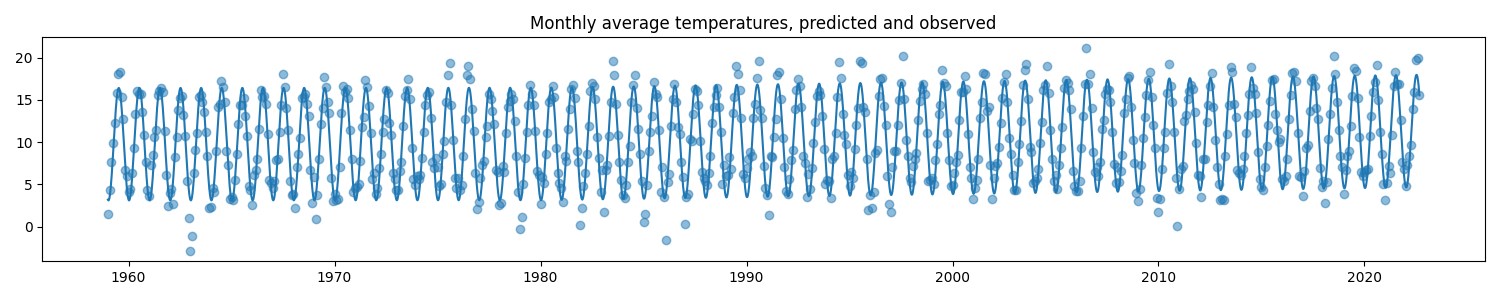
\includegraphics[width=0.8\textwidth]{q12_img}
\end{figure}

\item We are given a dataset with predictor $x$ and label $y$ and we fit the
linear model:

\[
y_i \approx \hat{\alpha} + \hat{\beta}x_i + \hat{\gamma}x^2_i
\]

After fitting the model using least squares estimation, we plot the
residuals $\epsilon_i = y_i - (\hat{\alpha} + \hat{\beta}x_i +
\hat{\gamma}x^2_i)$.

\begin{figure}[H]
    \centering
    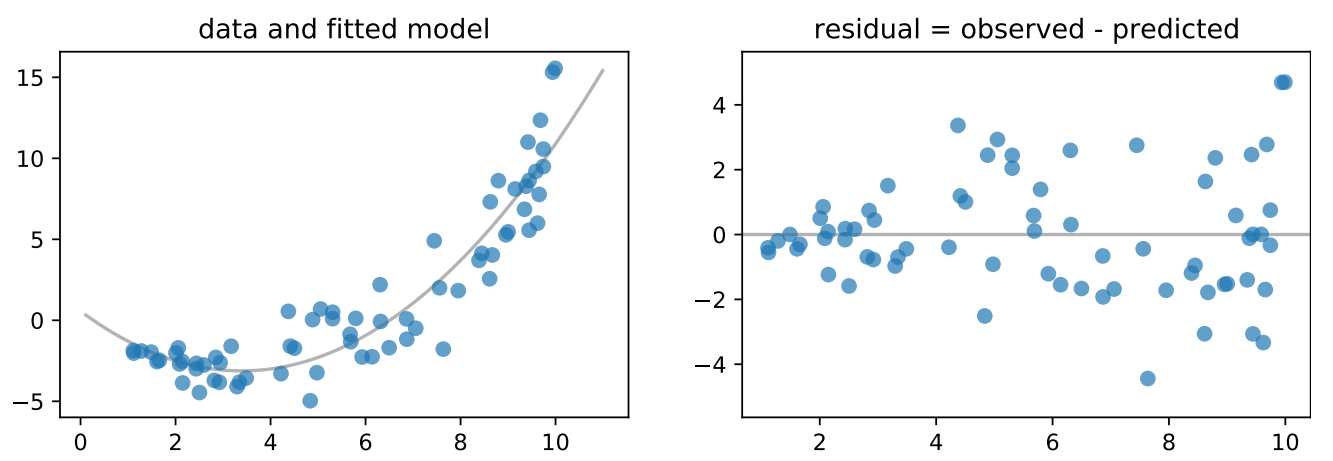
\includegraphics[width=0.8\textwidth]{q13_img}
\end{figure}

\begin{enumerate}[label=(\alph*)]

\item Describe what you would expect to see in the residual plot, if the
assumptions behind linear regression are correct.

I would expect residual error to be uncorrelated with $x$.

\item This residual plot suggests that perhaps $\epsilon_i \sim \mathcal{N}
(0, (\sigma x_i)^2)$ where $\sigma$ is an unknown parameter. Assuming this
is the case, give pseudocode to find the maximum likelihood estimators for
$\alpha$, $\beta$ and $\gamma$.

\begin{lstlisting}[language=Python]

url = "https://.../heteroscedasticity.csv"
hetero = pd.read_csv(url)

def predict(p):
	return p[0] + p[1] * hetero.x + p[2] * hetero.x ** 2

def logprobability(p):
	return np.sum(stats.norm.logpdf(hetero.y, predict(p), np.exp(p[3]) * hetero.x))

opt.fmin(lambda x: -logprobability(x), [0, -2, 0, -1])

\end{lstlisting}

\begin{figure}[H]
\centering
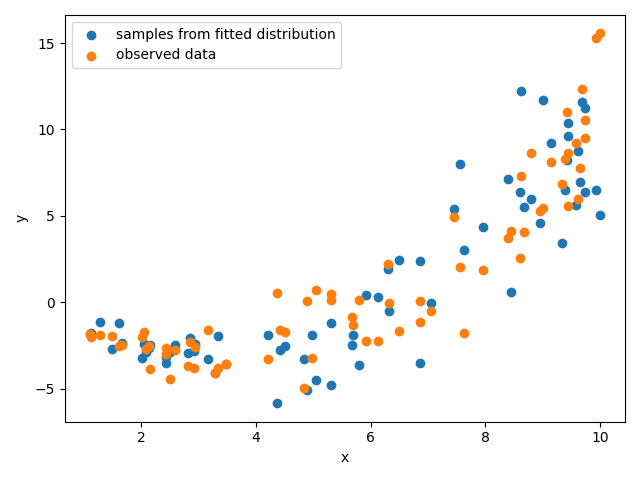
\includegraphics[width=0.5\textwidth]{./heterodistribution}
\end{figure}


\end{enumerate}

\item Let $(F_1, F_2, F_3, \dots) = (1, 1, 2, 3, \dots)$ be the Fibonacci
numbers, $F_n = F_{n-1} + F_{n-2}$. Define the vectors $f, f_1, f_2$ and
$f_3$ by

\[
\begin{split}
f 	&= [F_4, F_5, F_6, \dots, F_{m+3}] \\
f_1 &= [F_3, F_4, F_5, \dots, F_{m+2}] \\
f_2 &= [F_2, F_3, F_4, \dots, F_{m+1}] \\
f_3 &= [F_1, F_2, F_3, \dots, F_{m}] \\
\end{split}
\]

for some large value of $m$. If you were to fit the linear model

\[
f \approx \alpha + \beta f_1 + \beta f_2
\]

what parameters would you expect?

Because of the relationship $F_n = F_{n-1} + F_{n-2}$, the feature vectors
are not independent. Specifically $f = f_1 + f_2$.

So if we were to fit the model $f \approx \alpha + \beta f_1 + \beta f_2$, I
would expect the parameters to be $\alpha=0, \beta_1=1, \beta_2=1$.

What about the linear model

\[
f \approx \alpha + \beta f_1 + \beta f_2 + \beta_3 f_3
\]

There are two dependencies here. $f = f_1 + f_2$ and $f_1 = f_2 + f_3$.
Therefore the features are not linearly independent and so there is no
unique solution. However, for any solution to be optimum, the following
equations must hold: $\alpha = 0, \beta_1 + \beta_3 = 1, \beta_2 - \beta_3
= 1$.

\item For the police stop-and-search data from section 2.6, consider the model

\[
1[\text{outcome}=\text{find}] = \alpha + \sum^{}_{k\neq\text{White}} \beta_k
(1[\text{eth}=k] - 1[\text{eth}=\text{White}])
\]

Interpret the parameters.

\begin{itemize}

\item $\alpha$ is the probability of a white person being stop-and-searched

\item $\beta_k$ is the probability of a person of ethnicity
$k\neq\text{White}$ being stop-and-searched

\end{itemize}

\item Sketch the cumulative distribution functions for these two random
variables. Are they discrete or continuous?

\begin{lstlisting}[language=Python]

def rx():
	u = random.random()
	return 1/u

def ry():
	u2 = random.random()
	return rx() + math.floor(u2)

\end{lstlisting}

\begin{itemize}

\item $rx$

$rx$ is a continuous random variable with the following probability density
function:

\[
P(rx = x) =
\begin{cases}
0 & \ \text{if} \ x < 1 \\
\frac{2}{\ln 2} 2^{-x} & \ \text{if} \ x \geq 1 \\
\end{cases}
\]

Notice first that the probability that $rx < 2$ is equal to the probability
that $u \geq \frac{1}{2}$. Then notice the general case $P\left(rx <
2^x\right) = P\left(u > 2^{-x}\right) = 1 - 2^{-x}$. We can then
differentiate this general expression to get the probability density
function (note we only consider it over the valid domain $rx \geq 1$):

\[
\begin{split}
\text{pmf}(X) &= \pdv{P(X < x)}{x} \\
&= \frac{2}{\ln 2} 2^{-x} \\
\end{split}
\]

\begin{figure}[H]
\centering
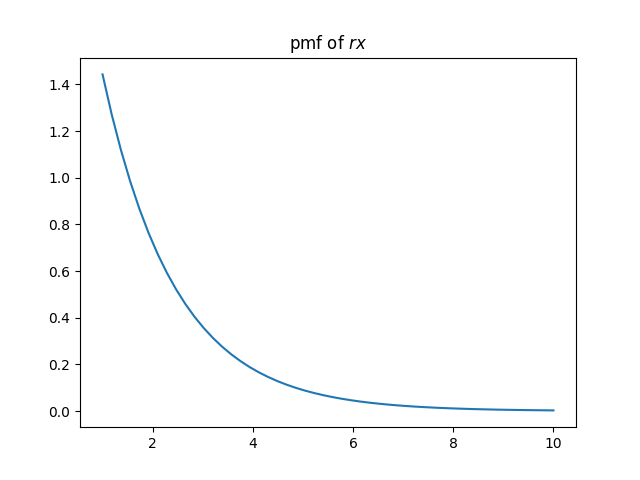
\includegraphics[width=0.5\textwidth]{./q16_rx_img}
\end{figure}

\item $ry$

$ry$ is a continuous random variable with the following probability density
function:

\[
P(ry = y) =
\begin{cases}
0 & \ \text{if} \ y < 1 \\
\frac{2}{\ln 2} 2^{-y} & \ \text{if} \ y \geq 1 \\
\end{cases}
\]

Note that this is the same as $rx$. \texttt{math.floor(u2)} will take the
floor of $u2$ -- for all $u2 < 1$ this will be zero. However, the probability
$u2 \geq 1$ is equal to the probability $u2 = 1$ -- which  is 0 as $u2$ is a
continuous distribution. Therefore the probability that $\texttt{math.floor}
(u2) = 1$ is also zero. Therefore $ry$ has the same distribution as $rx$.

\end{itemize}

\item Is it possible for a continuous random variable to have a probability
density function that approaches $\infty$ at some point in the support? Is
it possible to have this and also have finite mean and variance?

It is possible for a continuous random variable to have a probability
density function approaching $\infty$ for some point. It is also possible
for this variable to have finite mean and variance.

Consider the continuous random variable $X$ with probability density function:

\[
\text{pdf}_X(x) =
\begin{cases}
\frac{1}{2\sqrt{x}} & \ \text{if} \ 0 \leq x \leq 1 \\
0 & \ \text{otherwise} \\
\end{cases}
\]

Note firstly that $\lim_{x\rightarrow 0} \text{pdf}_X(x) = \infty$.

To prove $\text{pdf}_X$ is a valid probability density function, we have to
show it integrates to 1.

\[
\begin{split}
\int^1_0 \text{pdf}_X(x) \dd{x} &= \int^1_0 \frac{1}{2\sqrt{x}} \dd{x} \\
&= \left[ \sqrt{x} \right]^1_0 \\
&= 1 \\
\end{split}
\]
So this is a valid pdf which approaches $\infty$ at some point.

The mean is finite:
\[
\begin{split}
\bar{x} &= \int^1_0 x \cdot \text{pdf}_X(x) \dd{x} \\
&= \int^1_0 \frac{1}{2} \cdot \sqrt{x} \dd{x} \\
&= \left[ \frac{1}{3} x^{\frac{3}{2}} \right]^1_0 \\
&= \frac{1}{3} \\
\end{split}
\]

So the mean mean of $X$ is $\frac{1}{3}$ -- which is finite.

The variance is finite:

\[
\begin{split}
\text{Var}(x) &= \int^1_0 x^2 \cdot \text{pdf}_X(x) \dd{x} \dd{x} - \hat{x}^2 \\
&= \int^1_0 \frac{1}{2} \cdot x^\frac{3}{2} \dd{x} \dd{x} - \frac{1}{3}^2 \\
&= \left[ \frac{1}{5} \cdot x^{\frac{5}{2}} \right]^1_0 - \frac{1}{9} \\
&= \frac{1}{5} - \frac{1}{9} \\
&= \frac{4}{45} \\
\end{split}
\]

So the variance of $X$ is $\frac{4}{45}$ -- which is finite.

Therefore it is possible for a continuous random variable to have a pdf
approaching $\infty$ at some point, and to have a finite mean and variance.

\end{enumerate}

\begin{examquestion}{2018}{6}{8}

Fisher's Iris dataset contains, among other things, measurements of Petal
.Length and Sepal.Length for samples from each of three species of iris.
Suppose we want to fit the model

\[
\text{Petal.Length} = \alpha_s + \beta_s \text{Sepal.Length} + \mathcal{N}
(0, \sigma^2)
\]

where $s$ is the species.

\begin{enumerate}[label=(\alph*)]

\item Explain what is meant by ``linear model'', ``feature'' and
``orthogonal projection''. Rewrite the above model as a linear model made up
of linearly independent features and explain why they are linearly
independent.

A linear model is a model of the form $y_i \approx \sum^{n}_{i=1} k_i x_i $
for some response $y_i$, parameters $k_i$ and features $x_i$. Intuitively, a
linear model is a model which can be rewritten as a matrix multiplication.

A feature is an input variable. In the context of data science, a feature is
a dimension in the input vector.

An orthogonal projection is a projection of a response vector $\mathbf{y}$
into a feature space $(\mathbf{f}_1, \mathbf{f}_2, \dots, \mathbf{f}_n)$
such that all the features are linearly independent and there exist
constants $(\alpha_1, \alpha_2, \dots, \alpha_n)$ such that $\mathbf{y} =
\sum^n_{i=1} \alpha_i f_i$.

\[
\text{Petal.Length} \approx \sum^n_{s=1} \left(\alpha_s 1_{s=\text{species}} +
\beta_s
\text{Sepal.Length} 1_{s=\text{species}}\right)
\]

The features above are linearly independent because no feature is a linear
combination of any of the other features. For this particular dataset, you
can determine $1_{s=\text{species}}$ from $\text{Sepal.Length}
1_{s=\text{species}}$, however this is not a linear relationship and so the
features are linearly independent.

\item You are given a library function proj($y, [e_1, \dots, e_n]$). It
returns a list $[\lambda_1, \dots, \lambda_n]$ such that $\lambda_1 e_1 +
\dots + \lambda_n e_n$ is the orthogonal projection of the vector $y$ onto
the subspace spanned by vectors $\{e_1, \dots, e_n\}$. Explain what is meant
by the ``least squares method'' and give pseudocode using proj to find the
least squares estimators for $\alpha_s$ and $\beta_s$.

The ``least squares method'' minimises the sum of the squares of the
residuals (the differences between the prediction and the response). Least
squares can either be done mathematically or computationally.

\begin{lstlisting}[language=Python]

url = "https://.../iris.csv"

iris = pd.read_csv(url)

# if we use set then the order is not guai
species = list(sorted(set(iris['Species'])))

response = iris['Petal.Length']
features = []
for each in species:
	features.append(iris['Species'] == each)
	features.append((iris['Species'] == each) * df['Sepal.Length'])

features = np.array(features)

params = proj(response, features)

var = np.sum(np.power(features @ params - response, 2)) / response.shape[0]

sigma = np.sqrt(var)

\end{lstlisting}

The least squares estimator for $\alpha_{\text{species[i]}}$ is params[2 * i].\\
The least squares estimator for $\beta_{\text{species[i]}}$ is params[2 * i + 1].\\
The least squares estimator for $\sigma$ is sigma.

\item Explain how to compute the maximum likelihood estimators of $\alpha_s,
\beta_s$ and $\sigma$. In your answer, you should explain the relationship
between the least squares method and maximum likelihood estimation.

The mathematical method:

To find the maximum likelihood estimators for $\alpha_s$, $\beta_s$ and
$\sigma$ we need to form an expression for the probability of observing the
data that we did in terms of the parameters $\alpha_s$, $\beta_s$ and
$\sigma$. We should then form $n$ equations by differentiating with respect
to each of the parameters. This can then be solved like a simultaneous
equation and will form a closed form expression for each parameter. It may
be easier to use the logarithmic probability as it will remove all the
exponents created by the normal distribution. Note that we must optimise
over all parameters at the same time. If we do not, we will end up with
equations in terms of other parameters.

\[
\begin{split}
\Pr &= \prod^n_{i=1} \frac{1}{\sqrt{2\pi}\sigma} e^{-\frac{
\left(sum^n_{s=1}\alpha_s1_{s=\text{species}} + \beta_s\text{Sepal.Length}
1_{s=\text{species}} - \text{Petal.Length}\right)^2}{2\sigma^2}} \\
\ln \Pr &= \sum^n_{i=1} \left(\ln\frac{1}{\sqrt{2\pi}\sigma} -\frac{
\left(sum^n_{s=1}\alpha_s1_{s=\text{species}} + \beta_s\text{Sepal.Length}
1_{s=\text{species}} - \text{Petal.Length}\right)^2}{2\sigma^2}\right) \\
&= -\frac{n}{2}\ln 2\pi - n\ln \sigma - \left(\ln\frac{1}{\sqrt{2\pi}\sigma} -\frac{
\left(sum^n_{s=1}\alpha_s 1_{s=\text{species}} + \beta_s\text{Sepal.Length}
1_{s=\text{species}} - \text{Petal.Length}\right)^2}{2\sigma^2}\right) \\
\end{split}
\]

\[
\begin{split}
\pdv{\ln \Pr}{\alpha_s} = \dots \\
\pdv{\ln \Pr}{\beta_s} = \dots \\
\pdv{\ln \Pr}{\sigma} = \dots \\
\end{split}
\]

Then combine these equations and solve. The results will be the maximum
likelihood estimators for $\alpha_s$, $\beta_s$ and $\sigma$.

However, for many difficult datasets or complicated models, the maths can
become unmanageable. In these cases, it is often easier to determine maximum
likelihood estimators computationally.

The computational method:

Form an expression for the probability of our model generating the data that
has been observed in terms of $\alpha_s$, $\beta_s$ and $\sigma$. Then use a
numerical optimization function (such as \texttt{scipy.optimize.fmin}) to find 
the values of the parameters that maximise this probability. Note that we can
use a function that finds the minimum to find the maximum by minimizing the
negative. In almost all cases, we must use the logarithmic probabilities --
as the raw probability tends to zero very quickly (leading to floating point
precision errors). The parameters returned will be the maximum likelihood
estimators.

\begin{lstlisting}[language=Python]

response = iris['Petal.Length']
features = []
for each in species:
	features.append(iris['Species'] == each)
	features.append((iris['Species'] == each) * df['Sepal.Length'])

features = np.array(features)

def predict(x):
	return features @ x

def logprob(x):
	return np.sum(stats.norm.logpdf(response, predict(x[:-1]), np.exp(x[-1])))

opt.fmin(lambda x: -logprob(x), [...])

\end{lstlisting}

Finding the parameters such that the product of the normal probability density
functions between the predicted values and the response probabilities is
minimised (probability is maximised) is equivalent to finding parameters
that minimise the square of the difference between the response and the
prediction. Therefore least squares is equivalent to maximum likelihood
estimation over a normal distribution. If the residuals are distributed with
any distribution other than normal, this equivalence does not necessarily hold.

Assume we have some response vector $\mathbf{y}$ and predictions $\mathbf{x}$:

\[
\begin{split}
\Pr &= \prod \frac{1}{\sqrt{2\pi}\sigma} e^{-\frac{(\mathbf{x} - \mathbf{y})
^2}{2\sigma^2}} \\
\ln \Pr &= \sum -\frac{1}{2}\ln 2\pi - \ln \sigma - \frac{(\mathbf{x} -
\mathbf{y})^2}{2\sigma^2} \\
&= -\frac{n}{2}\ln 2\pi - n\ln \sigma - \sum\frac{(\mathbf{x} - \mathbf{y})
^2}{2\sigma^2} \\
\end{split}
\]

Maximising probability is equivalent to minimising the negative of the
logarithmic probability:

\[
\begin{split}
\ln\Pr &= \frac{n}{2}\ln 2\pi + n\ln \sigma + \sum\frac{(\mathbf{x} -
\mathbf{y})^2}{2\sigma^2} \\
\end{split}
\]

If we partially differentiate $\mathbf{x}$, we notice that the minima
of $\sigma$. Therefore maximising the probability is equivalent to
minimising $\sum(\mathbf{x} - \mathbf{y})^2$ -- the least squares method

Therefore, provided the residuals are distributed normally, the least
squares method is equivalent to maximum likelihood estimation.

\iffalse

Form an expression for the probability of generating the dataset. Then
partially differentiate to get $n$ expressions for MLE. We would be
better off using the logarithmic probability since the optimums are the
same and it simplifies the maths (less exponents). Then combine them all
into one and solve like a simultaneous equation. Note that we must optimise
over all parameters at the same time.

If you optimize over least squares then you get the distribution which
is also the one you'd find via maximum likelihood estimation.

\fi

\item We wish to know whether the $\beta_s$ coefficients for the three
species are noticeably different. Outline the Bayesian approach to answering
the question.


\iffalse

The Bayesian approach is to build a probability density function for the
distribution of the parameters. This distribution can be formed using Bayes
rule with a prior belief about the distribution of the parameters and the
observed results.

Critically, the distribution should be a joint probability distribution of
\textit{all} parameters. Additionally, we should be very careful not to make
the probability that a parameter has a certian value zero without
certainty that it is not that value. The prior distribution becomes less and
less important as we gather more data; however if the probability of a
parameter having a certain value is zero in the prior then it will remain
zero throughout.

Bayes' rule states that:

\[
\Pr(\beta; X) = \frac{p(\beta)\Pr(X; \beta)}{\Pr(X)}
\]

\begin{itemize}

\item $\Pr(\beta; X)$ is the probability distribution of $\beta$ given the
observed data $X$

\item $p(\beta)$ is the prior belief of the distribution of $\beta$

\item $\Pr(X; \beta)$ is the probability of the observed data given $X$

\item $\Pr(X)$ is the probability of the observed data occurring

\end{itemize}

This can be easily generalised to form a probability density function for
multiple parameters.

\[
\begin{split}
\Pr(\alpha, \beta; X) &= \frac{p(\alpha)p(\beta; \alpha)\Pr(X; \alpha,
\beta)}{\Pr(X)} \\
\Pr(\alpha, \beta, \sigma; X) &= \frac{p(\alpha)p(\beta; \alpha)p(\sigma;
\alpha,\beta)\Pr(X; \alpha, \beta, \sigma)}{\Pr(X)} \\
&\dots \\
\end{split}
\]

The Bayesian approach would approximate this distribution for all parameters.
The probability that the $\beta_s$ are the same is formed by
reparameterising the $\beta_s$ into a single parameter $\beta$ and then
integrating. IE the following equation:
\[
p_{\text{same}} = \int^{\infty}_{-\infty}
\int^{\infty}_{-\infty}\int^{\infty}_{-\infty}\int^{\infty}_{-\infty}\int
^{\infty}_0 \Pr(\beta, \alpha_{s_1}, \alpha_{s_2}, \alpha_{s_3}, \sigma)
\dd{\sigma} \dd{\alpha_{s_3}} \dd{\alpha_{s_2}} \dd{\alpha_{s_1}} \dd{\beta}
\]

The solution can be approximated computationally for example using
scipy.integrate or by a discrete approximation.

Integrating over 5 variables simultaneously is computationally difficult
and so in practice we would use a discrete approximation (computational Bayes)
or simplify the equation further.

\fi

The Bayesian approach is to build a probability distribution for the parameter
we are investigating. In this case, we are interested in the difference
between the parameters $\beta_{s_1}$, $\beta_{s_2}$ and $\beta_{s_3}$. Using
the Bayesian approach, we would therefore create a new parameter $\varepsilon$
defined as the maximum difference between the $\beta_{s_i}$ and build a
probability density function for this paremeter $\varepsilon$.

\[
\epsilon \triangleq \max\left(\left|\beta_{s_1} - \beta_{s_2}\right|,
\left|\beta_{s_1} - \beta_{s_3}\right|, \left|\beta_{s_2} -
\beta_{s_3}\right|\right)
\]

Given the dataset is moderately complicated, doing this analytically would
be impractical and therefore I would propose using Computational Bayes. In
Computational Bayes, we generate a large number of parameters according
to their prior distributions and then plot a histogram of the distribution 
of the parameter we are interested in, weighted by the probability of the
observed data occurring with that parameter.

Here is code which does what I have described:

\begin{lstlisting}[language=Python]

url = "https://.../iris.csv"
iris = pd.read_csv(url)

n = ...
means = [...]
stds  = [...]

def predict(x):
	sepal = np.array([iris['Sepal.Length']]).transpose()
	zip(range(3), ('setosa', 'versicolor', 'virginica'))
	return sum(map(lambda v:
		np.full((x.shape[0], iris.Species.size), iris.species == v[1]) *
		(x[:, 2 * v[0]] + sepal @ [x[:, 2 * v[0] + 1]]).transpose(),
		zip(range(3), ('setosa', 'versicolor', 'virginica'))))

def logprob(x):
	return np.sum(stats.norm.logpdf(np.full(
	(x.shape[0], iris.Species.size), iris['Petal.Length']).transpose(),
        predict(x).transpose(), np.exp(x[:, -1])), axis=0)

samples = stats.norm.rvs(np.full((n, len(means)), means), stds)

weights = logprob(samples)

weights = np.exp(weights + np.max(weights))

plt.xlim(0, 1)

plt.hist(np.maximum(np.abs(samples[:, 1] - samples[:, 3]),
                    np.abs(samples[:, 1] - samples[:, 5]),
                    np.abs(samples[:, 3] - samples[:, 5])),
                    weights=weights, density=True, bins=50)

plt.show()

\end{lstlisting}

The above code uses normal distributions for all prior distributions.

In the plot below I used $n=500000$ and the following parameters:
\begin{table}[H]
\centering
\begin{tabular}{c|c|c|c|c|c|c|c}
& $\alpha_{s_1}$ & $\beta_{s_1}$ & $\alpha_{s_2}$ & $\beta_{s_2}$ &
$\alpha_{s_3}$ & $\beta_{s_3}$ & $\sigma$ \\
\hline
$\mu$ & 0.8 & 0.1 & 0.2 & 0.7 & 0.6 & 0.8 & -1.4 \\
$\sigma$ & 0.2 & 0.2 & 0.2 & 0.2 & 0.2 & 0.2 & 0.1 \\
\end{tabular}
\end{table}

\begin{figure}[H]
    \centering
    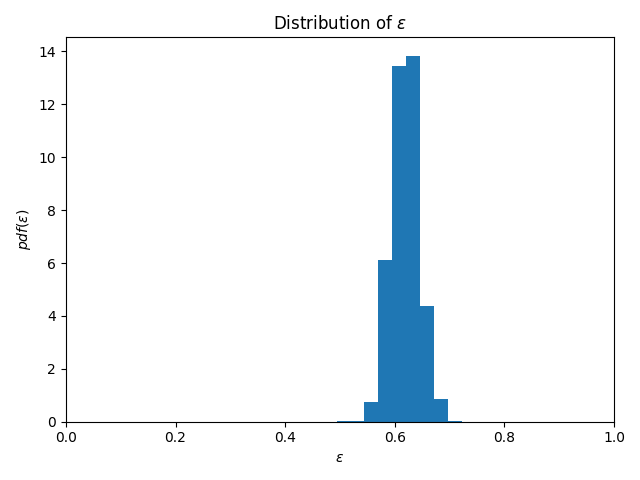
\includegraphics[width=0.5\textwidth]{./distribution_of_epsilon}
\end{figure}

\end{enumerate}

\end{examquestion}

\end{document}